\chapter{Event Reconstruction}
\label{c:recon}
% In this chapter the software and algorithms used to reconstruct particle physics objects are detailed. The idea is to work backwards from the information obtained from each of the sub-detectors to determine what particles passed through them.\\
% A software framework known as CMSSW has been developed in order to reconstruct the read out from the detector for each event


In Chapter~\ref{c:det}, each of the sub-detectors in CMS have been described; how particles interact with them and how electrical signals are read out. The next step is to combine the readouts from each detector in order to reconstruct the resulting particles from an interesting proton-proton collision. This snapshot of the collision output is known as an \emph{event}. An event will also contain PU from reconstructed particles from other simultaneous uninteresting collisions from the same or previous bunch crossing. Algorithms are used in order to subtract PU particles from the stored event. 
As a particle will usually traverse more than one sub-detector, it is advantageous to combine these outputs in order to reconstruct and identify the particle. This is achieved using the \emph{particle-flow} (PF) algorithm described in Section~\ref{sec:PF}. The objects which can be reconstructed using the PF algorithm such as muons, electrons, and jets are discussed in Sections~\ref{sec:muonreco},~\ref{sec:electronreco},~\ref{sec:jetreco} respectively. Further information can be obtained from these reconstructed objects such as how likely a jet is to have originated from a b-quark (Section~\ref{sec:btagreco}) and how the presence of neutrinos can be inferred by the imbalance of energy in the transverse plane of the detector (Section~\ref{sec:METreco}).  
The information from the detector is processed using a distributed computing infrastructure with custom software made by CMS, CMSSW.
% This chapter will discuss the main software used to reconstruct events from the detector read-out, CMSSW, and how a worldwide computer farm is used to process data.


% \section{Software}

% To-do:
% CMSSW, grid

\section{Track reconstruction}

Approximately 1000 charged particles are expected to traverse the CMS tracker at each bunch crossing at a PU of $\approx 20$ concurrent collisions. Each charged particle will interact with the silicon tracker as it continues through its trajectory from the collision point. Algorithms are designed to match hits in the tracker along each particle's trajectory in order to reconstruct its path so that information about the charge and momentum of the particle can be obtained. Not only is the tracker information used in offline reconstruction but it is used in the HLT, therefore it must have a fast response. Reconstructed paths from random particle hits in the tracker are considered to be \emph{fake tracks}~\cite{1748-0221-9-10-P10009}.\\
Knowledge of particle trajectories can help to pinpoint the collision vertex of interest which caused the trigger to fire. This is known as the \emph{primary vertex} and is described further in Section~\ref{sec:PVreco}. Accuracy in reconstructing tracks is essential for b-tagging as described in Section~\ref{sec:btagreco}.
Electrons lose energy through the tracker material in a non-gaussian way such that their tracks can not be fitted using the standard Kalman Filter. A Gaussian-Sum-Filter refit~\cite{GSF_Electron_Reconstruction_CMS}, which uses a sum of gaussians to estimate the energy loss, takes into account the interaction of electrons through the tracker material.


\section{Primary vertices \label{sec:PVreco}}

Primary vertices are the point at which the collision occurred, as opposed to secondary vertices which originate at the decay of subsequent particles coming from the collision. The first step in reconstructing primary vertices is to consider tracks which are consistent with the beam spot and cluster them into candidate vertices, separated along the z direction. Next a 3D fit is made and candidates which are compatible with originating from the beamline are kept~\cite{Caner1999118}. Primary vertices are ranked according to the sum of the momentum squared of all the tracks considered to have originated from that vertex. The vertex with the largest sum is regarded as the signal vertex, ie. the most interesting event, with higher momentum objects, that is most likely to have fired the trigger. 

\section{Particle-flow algorithm ~\label{sec:PF}}

The particle-flow (PF) algorithm combines information from all sub-detectors described in Section~\ref{c:det}, in order to improve the reconstruction of `final state' particles such as electrons, muons, photons, neutral hadrons and charged hadrons. Using this information more complicated higher-level objects, such as jets, can be reconstructed as described in the subsequent sections. Collections of different sub-detector objects, such as tracks or ECAL/HCAL hits, are created and each object is subsequently removed from each collection as they are identified as belonging to a final state particle within the algorithm.\\
The particle-flow algorithm reconstructs objects in an order starting from the easiest to reconstruct unambiguously. The hardest objects to reconstruct such as neutral hadrons are one of the last to be reconstructed because their properties can be constrained from the previously reconstructed objects.
The first objects to be reconstructed are PF muons. Each muon identified from the muon chambers is associated to compatible hits in the tracker. This associated track and muon chamber hits are then removed from their respective collection. The muon behaves like a minimum-ionising particle (MIP) in the ECAL and HCAL. With this assumption, energy can be subtracted from the ECAL, HCAL deposits (of the order of a few GeV) where the muon track is interpolated through these subdetectors.  Next, a Gaussian-Sum-filter refit is used to extrapolate electron candidate trajectories to the ECAL. On average, electrons have shorter trajectories than muons due to losing much of their energy through interactions with the tracker material. Tracker and ECAL variables are combined for the final identification of a PF electron after which the track and ECAL clusters are removed from their respective collections.\\
Charged hadrons are reconstructed from the remaining tracker, ECAL and HCAL deposits where the calorimeter hits are compatible with the tracker hits. Again, these hits are removed from the respective collections. Neutral hadrons leave no tracks in the tracker but have deposits in the ECAL and HCAL. Photons leave deposits in the ECAL but not the HCAL.\\


\section{Isolation \label{sec:isolation}}

Relative isolation (RelIso) is a measure of how isolated the muons or electrons are from surrounding hits in the detector from charged hadrons, neutral hadrons and photon energy which could contribute to a mis-measurement of their momentum. Only charged hadrons which are consistent with the signal primary vertex are considered in the calculation. As it is not possible to determine whether neutral hadrons are consistent with the signal primary vertex, instead the fact that the ratio of neutral hadronic to charged hadronic energy has been measured to be $\approx 0.5$ can be used\footnote{This is consistent with the $\pi^{0}$, $\pi^{+}$, and $\pi^{-}$ mesons (which constitute the majority of particles produced from p-p collisions) existing in an isospin triplet such that they have equal probability of being produced in a parton shower}. Hence the neutral hadronic energy in the transverse plane of the detector coming from the primary vertex, $E_{T,PV}^{NH}$, can be calculated as seen in Eq.~\ref{eqn:neutralE}, where $E_{T,sub}^{CH}$ is the transverse energy from charged hadrons which are associated to a sub-leading primary vertex and $E_{T,Tot}^{NH}$ is the total transverse neutral hadronic energy. 
% This is called the \emph{delta Beta correction}.
 The $max()$ function ensures that the corrected neutral hadronic energy is never defined as negative.


\begin{centering}
\begin{equation}
\Sigma E_{T,PV}^{NH}  =  max(0, \Sigma E_{T,Tot}^{NH} - 0.5\times \Sigma E_{T,sub}^{CH})
\label{eqn:neutralE}
\end{equation}
\end{centering}



The RelIso formula for muons, with the correction to neutral hadronic energy, can be found in Eq.~\ref{eqn:dBRelIso}. It is defined in a cone of radius $\textrm{R}=0.4$ and scaled by $1\; / \;\pt^{\mu}$ (where \pt is the momentum in the transverse plane of the detector) so that lower momentum muons are required to have less energy from hadrons and photons in the cone to be considered isolated.

\begin{centering}
\begin{equation}
RelIso = \left( \Sigma E_{T}^{CH} + \Sigma E_{T,PV}^{NH} +  \Sigma E_{T}^{\gamma} \right) \; / \;   \pt^{\mu}
\label{eqn:dBRelIso}
\end{equation}
\end{centering}


% Equation~\ref{eqn:dBRelIso} is used to define relative isolation for muons; 
For electrons RelIso is similarly defined, however, the neutral hadronic energy is estimated using a different method. The relative isolation for electrons is defined in Eq.~\ref{eqn:eRelIso} where EA denotes the Effective Area used in the analyses in this thesis. The EA is calculated by CMS from the average PU energy density per unit area in the $\rho$ ($\rho=\phi-\eta$) plane and the effective area based on shower shapes that has been measured by CMS (which depends on the $\eta$ value in the supercluster) for each event.

% \begin{centering}
% \begin{equation}
% C^{\rho} = \left( \Sigma E_{T}^{NH} + \Sigma E_{T}^{\gamma} - \rho\times\textrm{EA} \right) 
% \label{eqn:rhoCorr}
% \end{equation}
% \end{centering}

Equation~\ref{eqn:eRelIso} gives the RelIso formula for electrons with neutral hadronic energy correction where $\rho$ stands for the median density of pile-up contamination.

\begin{centering}
\begin{equation}
RelIso = \left( \Sigma E_{T}^{CH} + \Sigma E_{T}^{NH} + \Sigma E_{T}^{\gamma} - (\rho\times\textrm{EA}) \right) \; / \;   \pt^{e}
\label{eqn:eRelIso}
\end{equation}
\end{centering}

% \begin{centering}
% \begin{equation}
% RelIso = \left( \Sigma E_{T}^{CH} + C^{\rho} \right) \; / \;   \pt^{e}
% \label{eqn:eRelIso}
% \end{equation}
% \end{centering}

\section{Muons \label{sec:muonreco}}

It is important to be able to identify isolated muons coming from the signal process rather than from further decays from within jets or from mismatched tracks. Applying the identification criteria in Table~\ref{tab:muon_tight_cuts} can help to ensure a high purity of real muons is selected from the PF candidates described in Section~\ref{sec:PF}. Two working points (WP) are defined, tight and loose. Tight muons have tighter requirements on various quantities including \pt, as lower momentum muons are harder to distinguish from other particles. Tight muons are used when making selection requirements on how many muons should be in the event from the signal process. Loose muons are used to veto additional objects which are still likely to be muons but could be a misidentified object such as a pion. The loose criteria will capture more real muons in its selection but with a lower purity.
% but this is necessary when requiring a maximum number of muons in the event. 
The cut values for each working point are given in Table~\ref{tab:muon_tight_cuts} for the 8 TeV analysis and the 13 TeV analysis.

The transverse impact parameter in the $\phi$-plane with respect to the leading primary vertex is denoted as d0 in the table. The distance between the leading primary vertex and the muon track in the z-direction is denoted dz. These two variable can be used to establish how consistent the muon track is with the leading primary vertex.
A \emph{Global Muon} is a muon which has been identified from both hits in the muon chamber and hits in the tracker whereas a \emph{Tracker Muon} has only been identified from tracker hits.


\begin{table}[htpb!]
\footnotesize
\begin{center}
\begin{tabular}{|r|c|c|c|c|}
\hline
\multicolumn{1}{|l|}{}                                          & \multicolumn{2}{c|}{Tight WP} & \multicolumn{2}{c|}{Loose WP} \\ \cline{2-5} 
Requirements                                                    & 8 TeV         & 13 TeV        & 8 TeV         & 13 TeV        \\ \hline
Is a Global Muon and a Tracker Muon                               & yes           & yes           & yes           & yes           \\
\pt (\GeV)                                                     & $>$30            &$>$ 26            & $>$10            &$>$ 10            \\
$\lvert \eta \rvert$                                          &  $<$2.1           &  $<$2.1           &  $<$2.5           &  $<$2.5           \\
RelIso                                                    &  $<$ 0.12          & $<$  0.15          & $<$  0.2           &  $<$ 0.25          \\
Number of valid hits in the tracker                          & $>$5             & $>$5             & -             & -             \\
Number of hits in the muon stations                          & $>$0             & $>$0             & -             & -             \\
d0 (cm)  & $<$0.2           & $<$0.2           & -             & -             \\
dz (cm)       & $<$ 0.5           & $<$ 0.5           & -             & -             \\
Number of hits in the  pixel tracker                          & $>$0             & $>$0             & -             & -             \\
Normalised $\chi^{2}$ of track                              & $<$ 10            &$<$  10            & -             & -             \\
Number of muon stations matched to track                       &  $>$1             &  $>$1             & -             & -             \\ \hline
\end{tabular}
\caption{The cuts used for the tight and loose muon identification at 8 TeV~\cite{muonIDtwikieight} and 13 TeV~\cite{muonSFtwiki}.}
\label{tab:muon_tight_cuts}
\end{center}
\end{table}



\section{Electrons \label{sec:electronreco}}

In this thesis the word electron is mostly used to include both charges, electron and positron. Electrons typically lose a large fraction of their energy in the tracker material via Bremsstrahlung. This is one of the biggest challenges in reconstructing electrons as the Bremsstrahlung radiation needs to be taken into account to accurately measure their momentum. These Bremsstrahlung photons can also convert into electron-positron pairs in the tracker material creating secondary electrons which must be distinguished from the signal electrons coming from the hard process. 

Similar to the muon reconstruction, two working points are defined for electrons from the PF candidates. Tight electrons are used when requiring electrons as part of the signal process and a looser set of criteria are used in order to veto on extra electrons in the event ensuring a strict selection. The loose selection will contain more electrons but with a lower purity. 

There are multiple ways to identify electrons, two of which are used in this thesis. At 8 TeV a multivariate technique to identify electrons was used. At 13 TeV a \emph{cuts based identification} was used as the electron tools from CMS were not as advanced by the time the analysis was performed.

The tight and veto working points at $\sqrt{s}=8$ TeV can be found in Table~\ref{tab:electron_tight_cuts8}. The multivariate algorithm used for electron identification assigns a discriminator value which is closer to one for candidate particles which are more consistent with being a real electron and closer to zero if not. This discriminator is shown in Fig.~\ref{fig:mvaeid}. A conversion veto is applied for tight electrons which mitigates against identifying electrons which have come from photons converting into an electron-positron pair in the detector~\cite{Khachatryan:2015hwa}.


\begin{figure}[ht!]
\begin{center}
    \includegraphics[width=0.49\textwidth]{images/NonTrigBDTeBarrel.pdf}
    \includegraphics[width=0.49\textwidth]{images/NonTrigBDTeEndcap.pdf}
    \caption{Output of the electron-identification boosted decision tree (BDT) multivariate algorithm for non-triggering electrons from Z$~\rightarrow~$e$^{+}$e$^{-}$ data (black dots) and simulated(solid histograms) events, and from background-enriched events in data (triangles), in the ECAL a) barrel (left) and b) endcaps (right).  For triggering electrons, to mimic the requirements applied at the HLT loose, ientification and isolation requirements are applied as a preselection~\cite{Khachatryan:2015hwa}.}
    \label{fig:mvaeid}
\end{center}
\end{figure}

\begin{table}[htpb!]
\footnotesize
\begin{center}
\begin{tabular}{|r|c|c|}
\hline
Requirements   & Tight & Veto \\ \hline
\ET (GeV) & $>$30    & $>$20   \\
$|\eta| $  & $<$2.5   & $<$2.5  \\
$|$d$0|$ (cm) & $<$0.02  & -    \\
ConversionVeto & yes   & -    \\
MVA ID & $>$  0.9   &$>$   0    \\
RelIso   & $<$0.1   & $<$0.2  \\ \hline
\end{tabular}
\caption{The cuts used for the tight and veto electron identification at $\sqrt{s}=8$~TeV~\cite{electronIDeight}.}
\label{tab:electron_tight_cuts8}
\end{center}
\end{table}

The tight and veto working points are given for the barrel and endcap in Table~\ref{tab:electron_tight_cuts13} for the $\sqrt{s}=13$~TeV analysis. The ECAL crystal that contains the largest energy deposit is considered to be the \emph{seed crystal}. Strips of ECAL crystals (in $\phi$) are clustered together to create a ``supercluster'' (SC) with minimum requirements on initial seed crystal energy, as well as minimum energy of each strip. The distances in $\eta$ and $\phi$ between the supercluster and the point in the ECAL where the track from the PV is extrapolated to, are defined as $\Delta \eta_{In}$ and $\Delta \phi_{In}$, respectively. The ratio of the hadronic to electromagnetic energy around the seed cluster is denoted $\frac{h}{E}$. Photons which come from conversions often have tracks which do not pass through the innermost layer of the tracker, therefore limits are set on the number of expected missing hits, $N_{miss}$. The effect of the momentum loss through the tracker material can be quantified in the variable $\frac{1}{E_{SC}} - \frac{1}{p}$, where $E_{SC}$ is the energy of the supercluster and $p$ is the momentum of the track at closest approach to the vertex. The shower shape variable, $\sigma_{I_{\eta}I_{\eta}}$, describes the lateral extension of the shower along the $\eta$ direction.

\begin{table}[htpb!]
\footnotesize
\begin{center}
\begin{tabular}{|r|c|c|c|c|}
\hline
& \multicolumn{2}{c|}{Tight} & \multicolumn{2}{c|}{Veto} \\
\cline{2-5}
%&Tight & TIght & Veto & Veto \\
Requirements &  Barrel        &   Endcap  &  Barrel        &   Endcap  \\
%&  ($|\eta_{SuCluster}|< 1.4442$)         &   ($1.5660<|\eta_{SuCluster}|<2.5$)  &  ($|\eta_{SuCluster}|< 1.4442$)         &   ($1.5660<|\eta_{SuCluster}|<2.5$)  \\
\hline
$\sigma_{I_{\eta}I_{\eta}} $ & $ <$0.0101 & $ <$0.0279 & $ <$0.0114 & $ <$0.0352\\
$|\Delta \eta_{In}| $  & $ <$0.00926 &$ <$ 0.00724  & $ <$0.0152 & $ <$0.0113  \\
$|\Delta \phi_{In}|  $  &  $<$0.0336 & $<$0.0918 & $<$ 0.216 & $<$0.237  \\
$\frac{h}{E} $ &$<$0.0597 & $<$0.0615  &$<$0.181 & $<$0.116  \\
RelIso & $\leq$0.0354 & $\leq$0.0646& $\leq$0.126 & $\leq$0.144\\
$\frac{1}{E_{SC}} - \frac{1}{p}$ (GeV)$^-1$ & $<$ 0.012 & $<$ 0.00999  & $<$ 0.207 & $<$ 0.174 \\
$|$d$0| < $  & $<$0.0111 & $<$0.0351  & $<$0.0564 & $<$0.222\\
$|$dz$| $  & $<$0.0466 & $<$0.417 & $<$0.472 & $<$0.921\\
$N_{miss}$  & $\leq$2 & $\leq$1 & $\leq$2 & $\leq$3  \\
pass conversion veto & yes & yes& yes & yes  \\
\hline
\end{tabular}
\caption{The cuts used for the tight and veto electron identification at $\sqrt{s}=13$~TeV~\cite{electronID} where barrel is $|\eta_{SC}|< 1.4442$ and endcap is  ($1.5660<|\eta_{SC}|<2.5$)}
\label{tab:electron_tight_cuts13}
\end{center}
\end{table}

Electron reconstruction can not be performed accurately in the transition region ($TR$) between the ECAL barrel and endcap, $1.4442<TR<1.5660$ and hence they are excluded from physics analyses.

\section{Jets \label{sec:jetreco}}
When partons such as quarks and gluons hadronise, they form a number of charged and neutral hadrons travelling in approximately the same direction of travel as the original parton. These final state particles can be clustered into what is known as a \emph{jet} using the anti-$\kappa_{\textrm{T}}$ reconstruction algorithm~\cite{Cacciari:2008gp}. This is an infrared and collinear safe algorithm which starts with a high \pt `seed' deposit in the calorimeter and uses the distance measure in Eq.~\ref{eqn:antikt1} to find the nearest deposit to merge with. If the distance between the seed particle and the beam, $d_{iB}$ in Eq.~\ref{eqn:antikt2}, is smaller than the distance to another hit, $d_{ij}$, the particle is merged with the beam~\cite{Salam2010}. Otherwise, the particle is merged with the nearest hit, according to $d_{ij}$. The algorithm terminates when $d_{iB}<d_{ij}$ and the merged particles are considered to be a jet. In this thesis, a distance parameter of $R = 0.5~\left(0.4\right)$ is used to reconstruct jets in the \runone (\runtwo) analysis in Chapter~\ref{c:Run1}~(\ref{c:Run2}). The distance parameter was changed for \runtwo to be consistent with the ATLAS experiment and to mitigate against PU contamination. 


\begin{equation}
d_{ij}=min\left( p_{\textrm{T}i}^{~-2},p_{\textrm{T}j}^{~-2} \right) \frac{\Delta R_{ij}^{2}}{R^{2}} \textrm{ , where } \Delta R_{ij}^{2} = {\left( y_{i} - y_{j}\right)}^{2} +  {\left( {\phi}_{i} - {\phi}_{j}\right)}^{2}
\label{eqn:antikt1}
\end{equation}

\begin{equation}
d_{iB}=p_{\textrm{T}i}^{2}
\label{eqn:antikt2}
\end{equation}

Corrections are applied to the jet energy to account for the non-uniform response of the detector in \pt and $\eta$. The first correction is the \emph{L1FastJet} correction which is applied to both data and simulation to remove the energy coming from PU events. The \emph{L2Relative} and \emph{L3Absolute} corrections respectively correct for the non-uniform response in $\eta$ and \pt for both data and simulation. The \emph{L2L3Residual} corrections are applied to simulation only and correct the remaining small differences in jet response between data and simulation such as correcting the jet absolute scale (JES). The jet energy resolution (JER) is also smeared by 10$\%$ as the resolution is worse in data than in simulation. Together these corrections are called the \emph{jet energy corrections}~(JEC)~\cite{Khachatryan:2016kdb}.
Jet identification critera are applied to suppress fake jets arising from electrons showering in the ECAL due to Bremsstrahlung. This includes requiring $|\eta|<2.5$, \pt$>30$~GeV and a separation from the nearest loose muon or electron of $\Delta R>0.4$.

The biggest gains in using the PF algorithm come from performing the jet reconstruction on PF particles. The jet-matching efficiency, jet energy resolution and the reconstruction of the jet \pt are improved compared to using calorimeter information alone~\cite{CMS-PAS-PFT-10-001}.

\section{b-tagging ~\label{sec:btagreco}}
The presence of jets in an event indicate that the particles emerging from the collision include quarks and gluons. Being able to identify or \emph{tag} which flavour of quark hadronised in the detector is extremely useful for a wide range of analyses. Particularly for searches for final states containing four top quarks, the ability to identify b-quarks originating from the decay of top quarks is incredibly beneficial in allowing us to discriminate between the signal and backgrounds. 
 % $\Lambda_{B}$
The particle shower coming from the hadronisation of b-quarks will contain B mesons and $\Lambda_{B}$ (and other) baryons. These particles travel further in the detector due to having longer decay times than light flavour (u, d, s) mesons and baryons, resulting in a typical flight distance of up to a few centimetres~\cite{Collaboration2015BS0}. The \emph{impact parameter} (IP), defined as the distance between the primary vertex and the extrapolated point of closest approach of a track, will be larger for tracks coming from the decay of a hadron containing a b-quark. The tracks emerging from this decay can form a secondary vertex. This information is exploited in the Combined Secondary Vertex (CSV) algorithm~\cite{Chatrchyan:2012jua}. The CSV algorithm is used to identify or \emph{tag} jets which originate from b-quarks by assigning a discriminator value between 0 and 1, where larger values are more consistent with b-quark jets. Loose (CSVL), medium (CSVM) and tight (CSVT) working points are defined at values of the discriminator for a given mis-identification rate. For analyses at $\sqrt{s} = 13$~TeV the algorithm was improved and is called Combined Secondary Vertex version 2 algorithm (CSVv2)~\cite{CMS-PAS-BTV-15-001}, the output of which is shown in Fig.~\ref{fig:CSVv2}. Working points, selection efficiencies for b-quarks and mis-identification rates are given in Table~\ref{tab:btag}.

\begin{figure}[ht!]
\begin{center}
    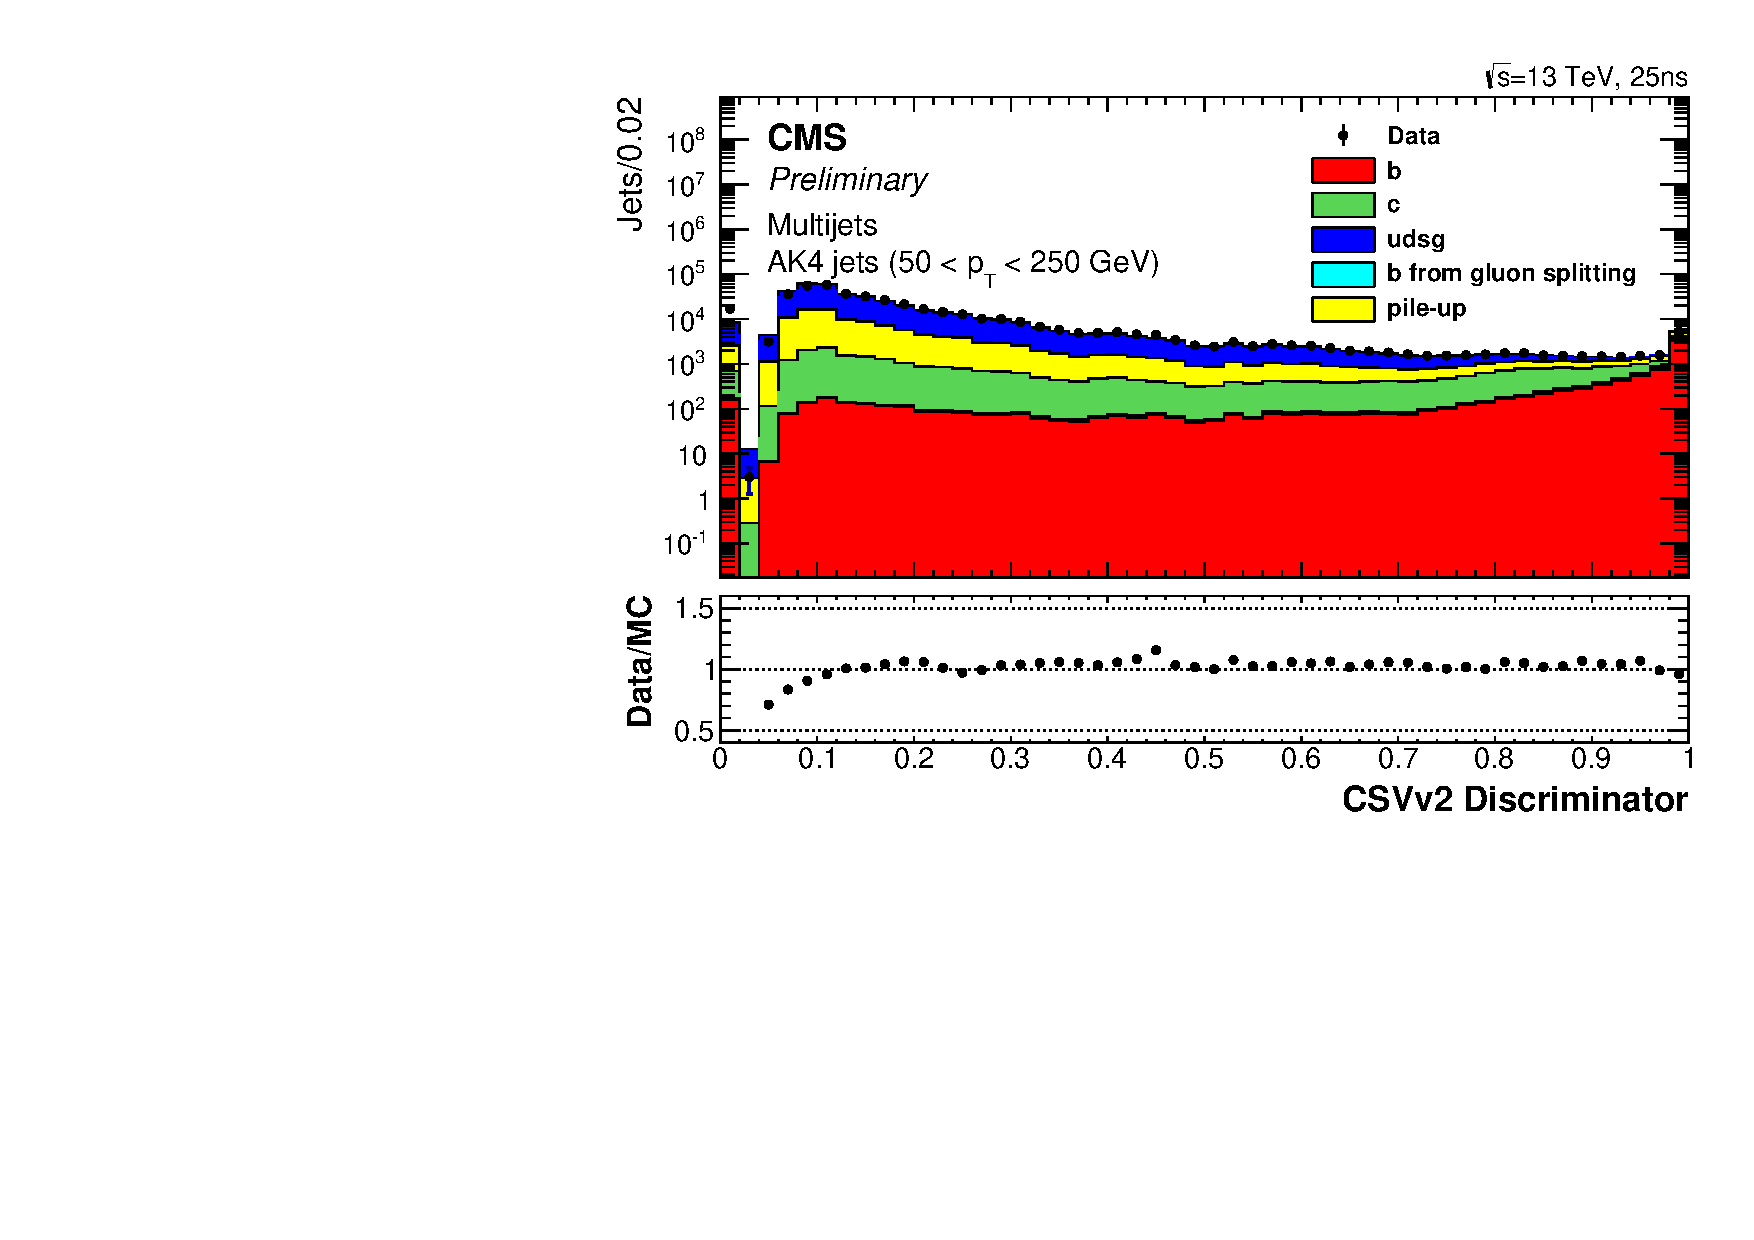
\includegraphics[width=0.99\textwidth]{images/btagCSV.pdf}
    \caption{CSVv2 discriminator distribution at $\sqrt{s}=13$~TeV using a multi-jets sample. Jets are reconstructed using the \antikt algorithm with $R=0.4$~\cite{CMS-PAS-BTV-15-001}.}
    \label{fig:CSVv2}
\end{center}
\end{figure}
% \footnote{This efficiency was measured using the TTJets MLM sample for the medium working point at $\sqrt{13}$ TeV. The CSVv2L and CSVv2T efficiences have been taken from here~\cite{btageff} }.

\begin{table}[htpb!]
\footnotesize
\begin{center}
\begin{tabular}{l|l|c|c|c}
$\sqrt{s}$ (TeV)    & Name   & \multicolumn{1}{l|}{WorkingPoint} & \multicolumn{1}{l|}{Selection Efficiency ($\%$)} & \multicolumn{1}{l}{Mis-identification ($\%$)} \\ \hline
\multirow{3}{*}{8}  & CSVL   & 0.244                             & $<$80                                                 & 0.1                                               \\ \cline{2-5} 
                    & CSVM   & 0.679                             & $<$62                                                 & 0.01                                   \\ \cline{2-5} 
                    & CSVT   & 0.898                             & $<$35                                               & 0.001                                               \\ \hline
\multirow{3}{*}{13} & CSVv2L & 0.46                              & 82                                               & 11.5                                          \\ \cline{2-5} 
                    & CSVv2M & 0.8                               & 67                                               & 1.4                                           \\ \cline{2-5} 
                    & CSVv2T & 0.935                             & 47                                               & 0.15                                         
\end{tabular}
\caption{b-tagging working points and their selection and mistagging efficiencies for PF jets.}
\label{tab:btag}
\end{center}
\end{table}


\section{Missing transverse energy ~\label{sec:METreco}}
As it is not possible to detect neutrinos and potentially some BSM particles because they interact incredibly weakly with matter, their existence can be inferred by examining the sum of the momentum of particles in the transverse plane of the detector. The transverse plane is defined to be transverse to the beamline. Starting with the assumption that the total momentum in the transverse plane is zero., an imbalance in the sum of the momentum of detectable particles is considered to be missing transverse energy (\ETmiss), as defined in Eq.~\ref{eqn:MET}. Tthe \pt of jets is used after the JEC have been applied~\cite{CMS:2016ljj}.
\begin{equation}
\ETmiss = ~- \sum_{\textrm{all particles,}i} \hat{ {p}_{\textrm{T},i} }
\label{eqn:MET}
\end{equation}


